
\documentclass{article}
%\usepackage[utf8]{inputenc}
%\usepackage[a4paper, total={7in, 8in}]{geometry}
\usepackage[left=15mm,top=26mm,right=8mm,bottom=15mm]{geometry}

\usepackage{spverbatim}
\usepackage{minted}
\usepackage{amssymb}
\usepackage{bm}
\usepackage{graphicx}
\usepackage{amsmath}

%\setlength{\voffset}{-0.75in}
%\setlength{\headsep}{-10pt}


\title{EECE 5639- Homework 3}
\author{Sreejith Sreekumar: 001277209}
\date{\today}
\begin{document}

\maketitle

\section*{Question 1}

\begin{minted}{Matlab}

  %Creating the image in the question
  function image = get_image()
    image = zeros(8, 8);
    
    for x = 1:8
        for y = 1:8
            image(x,y) = abs(x-y);
        end
    end
  end
\end{minted}

\subsection*{Prewitt Mask}
\begin{minted}{Matlab}
  [PGmag, PGdir] = imgradient(image,'prewitt');
  disp(PGmag);
  disp(PGdir);

  % Output - Disregarding boundaries

        % Gradient Magnitude
  
             0    5.6569    8.4853    8.4853    8.4853    8.4853    
        5.6569         0    5.6569    8.4853    8.4853    8.4853    
        8.4853    5.6569         0    5.6569    8.4853    8.4853    
        8.4853    8.4853    5.6569         0    5.6569    8.4853    
        8.4853    8.4853    8.4853    5.6569         0    5.6569    
        8.4853    8.4853    8.4853    8.4853    5.6569         0   

        % Gradient Orientation


                0   45.0000   45.0000   45.0000   45.0000   45.0000   
        -135.0000         0   45.0000   45.0000   45.0000   45.0000   
        -135.0000 -135.0000         0   45.0000   45.0000   45.0000   
        -135.0000 -135.0000 -135.0000         0   45.0000   45.0000   
        -135.0000 -135.0000 -135.0000 -135.0000         0   45.0000   
        -135.0000 -135.0000 -135.0000 -135.0000 -135.0000         0   
\end{minted}

\pagebreak

\subsection*{Sobel Mask}

\begin{minted}{Matlab}
  [SGmag, SGdir] = imgradientxy(image);
  disp(SGmag);
  disp(SGdir);

  % Output - Disregarding boundaries

        % Gradient Magnitude

             0     6     8     8     8     8     
            -6     0     6     8     8     8     
            -8    -6     0     6     8     8     
            -8    -8    -6     0     6     8     
            -8    -8    -8    -6     0     6     
            -8    -8    -8    -8    -6     0     


        % Gradient Orientation            

            0    -6    -8    -8    -8    -8    
            6     0    -6    -8    -8    -8    
            8     6     0    -6    -8    -8    
            8     8     6     0    -6    -8    
            8     8     8     6     0    -6    
            8     8     8     8     6     0    
\end{minted}

\begin{figure}
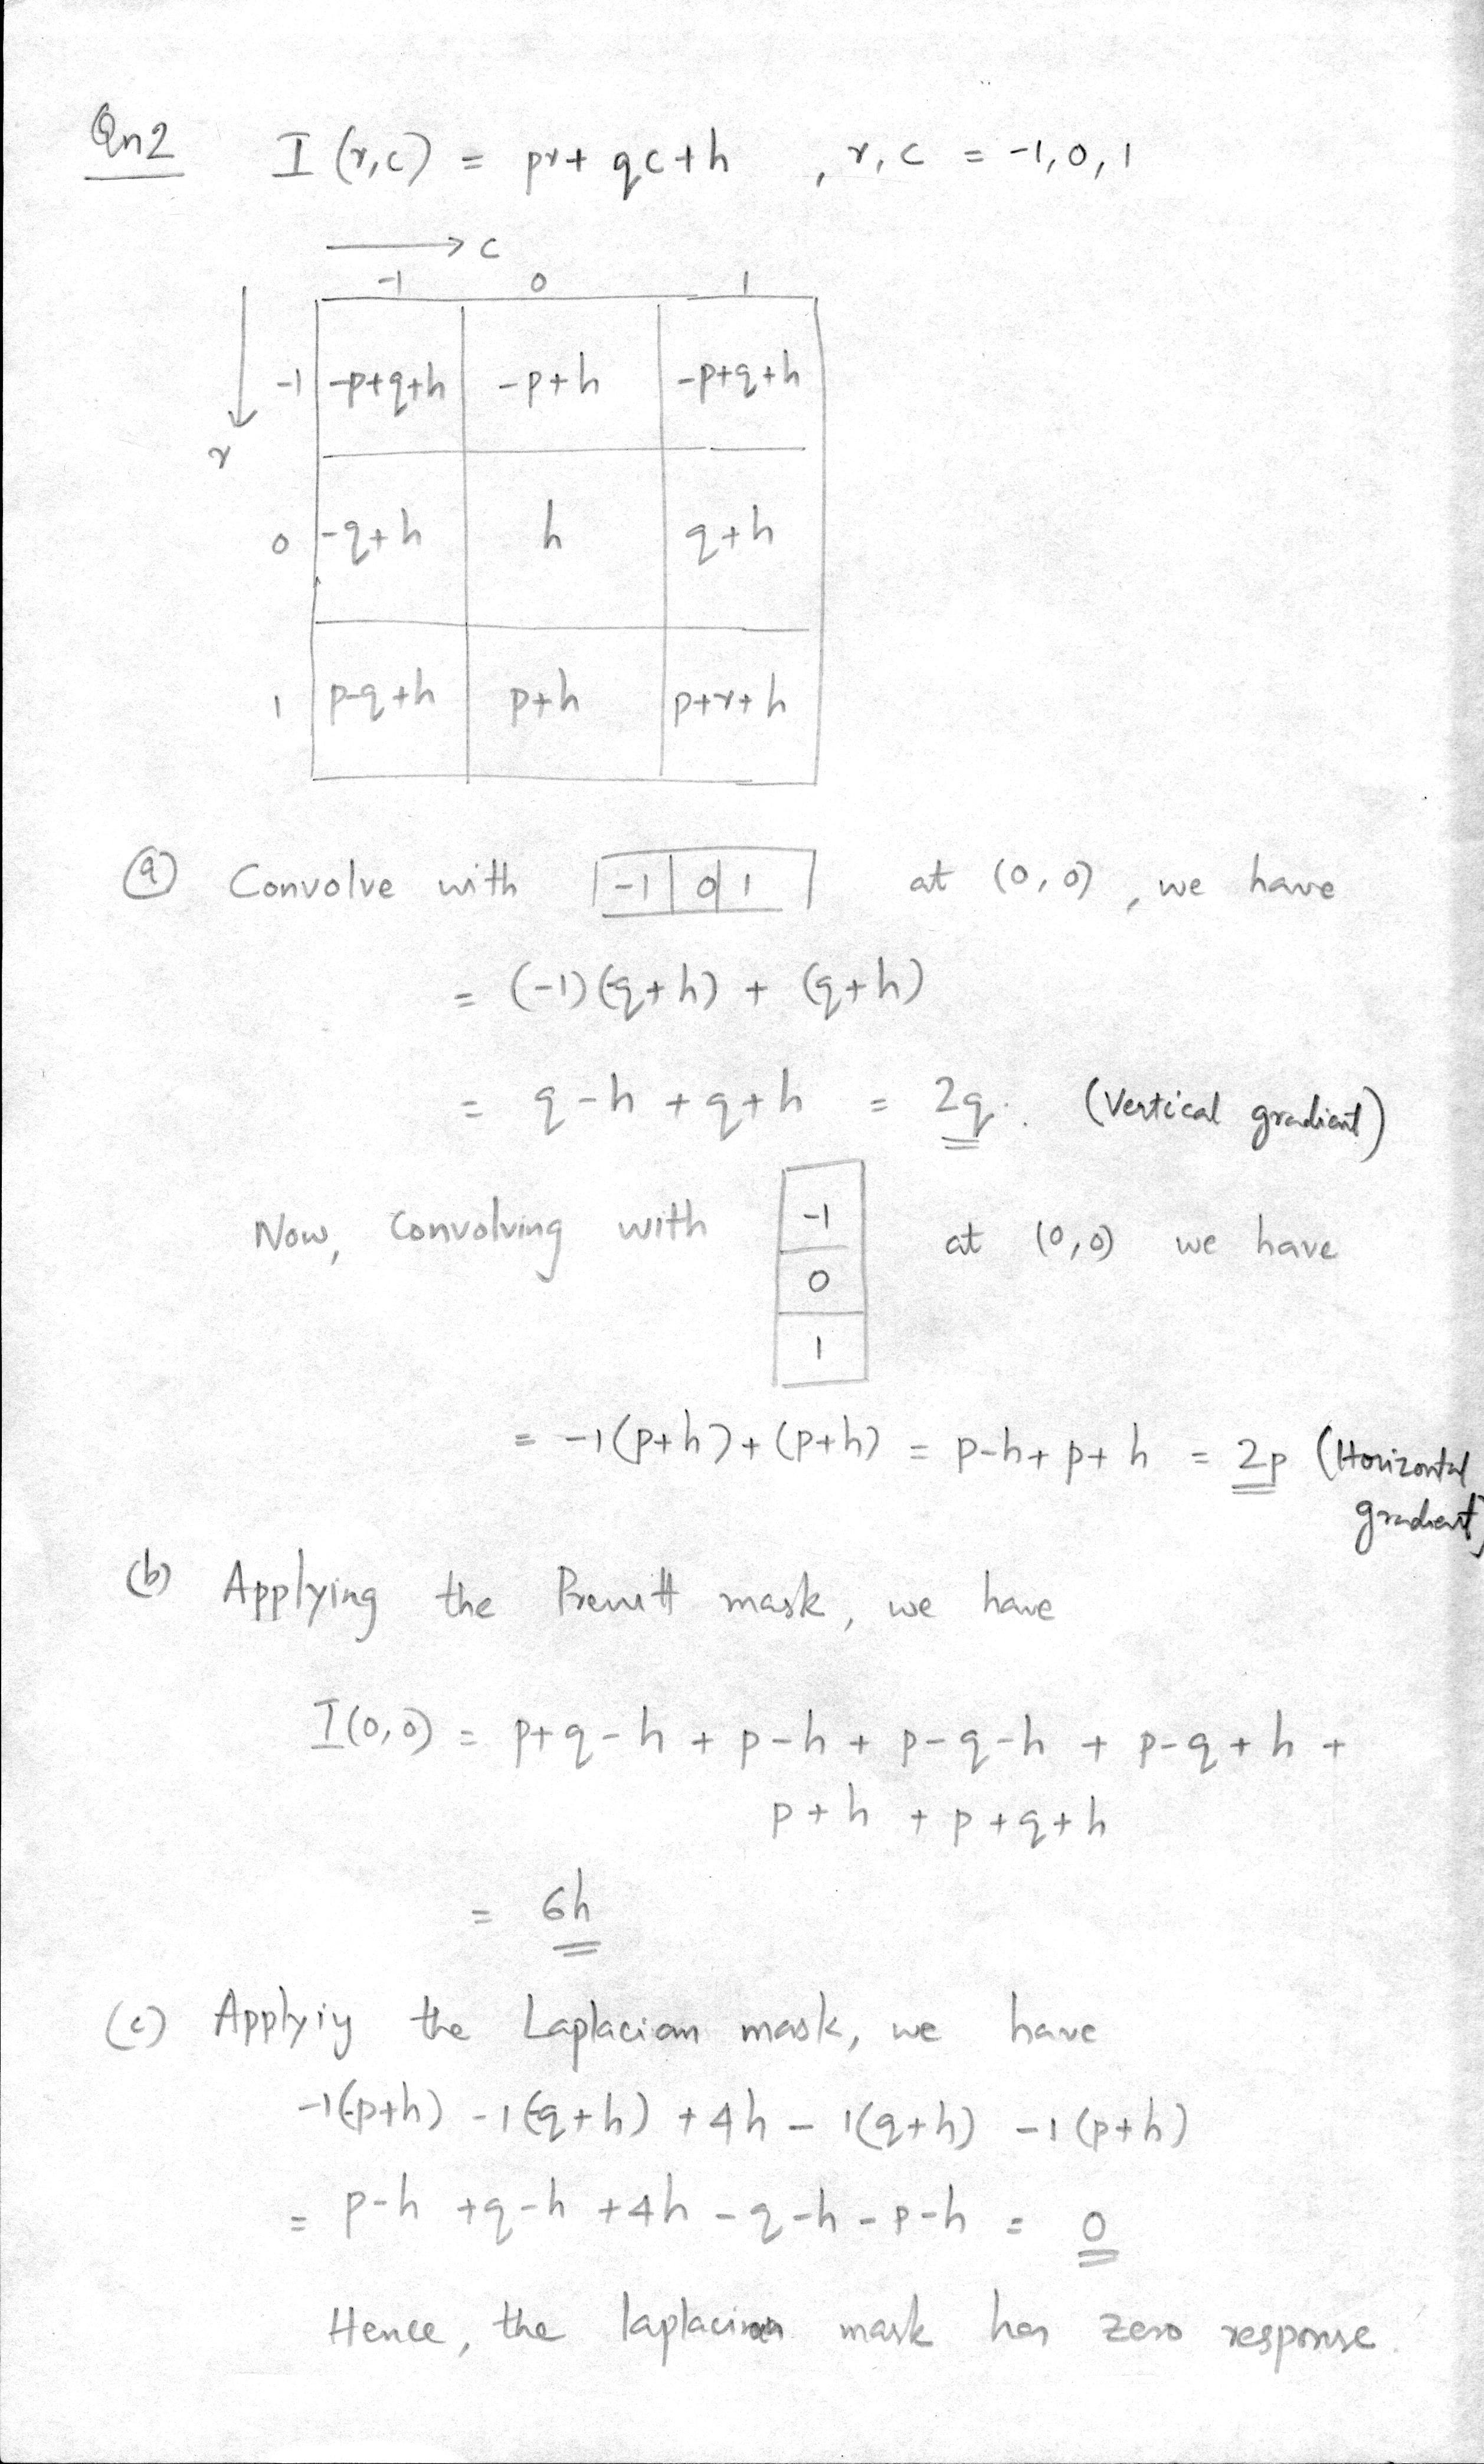
\includegraphics[width=15cm]{qn2.jpg}
\end{figure}

\pagebreak

\section*{Question 3}

\begin{minted}{Matlab}

function image = get_image_with_corners()
    image = zeros(21,20);
    for x = 11:21
        for y = 1:10
            image(x,y) = 40;
        end
    end
    
    for x = 1:10
        for y = 11:20
            image(x,y) = 40;
        end
    end    
end

img2 = get_image_with_corners();

% Gradient in X - direction
maskx = [-1 -1 -1;0 0 0;1 1 1];
Gx = conv2(img2, maskx);

% Gradient in Y - direction
masky = [-1 0 1;-1 0 1;-1 0 1];
Gy = conv2(img2, masky);


Ex2  = Gx.*Gx;
Ey2  = Gy.*Gy;
ExEy = Gx.*Gy;

% Build the C Matrix from the Ex, Ey and ExEy matrices

function matrix = CreateCMatrix(Ex2, Ey2, ExEy, i, j)
    matrix = zeros(2,2);
    matrix(1,1) = Ex2(i-1, j-1) + Ex2(i-1, j) + Ex2(i-1, j+1) + ...
        + Ex2(i, j-1) + Ex2(i,j) + Ex2(i,j+1) + Ex2(i+1,j-1) + Ex2(i+1,j) + Ex2(i+1,j+1);
    matrix(1,2) = ExEy(i-1, j-1) + ExEy(i-1, j) + ExEy(i-1, j+1) + ...
        + ExEy(i, j-1) + ExEy(i,j) + ExEy(i,j+1) + ExEy(i+1,j-1) + ExEy(i+1,j) + ExEy(i+1,j+1);
    matrix(2,1) = matrix(1,2);
    matrix(2,2) = Ey2(i-1, j-1) + Ey2(i-1, j) + Ey2(i-1, j+1) + ...
        + Ey2(i, j-1) + Ey2(i,j) + Ey2(i,j+1) + Ey2(i+1,j-1) + Ey2(i+1,j) + Ey2(i+1,j+1);
end


CMatrix = zeros(2,2,21,20);


% Excluding borders while summing
for i=2:20
    for j=2:19
       CMatrix(:,:,i,j) = CreateCMatrix(Ex2, Ey2, ExEy, i, j); 
    end
end        


% Finding those values for which CMatrix has Sum(Ex^2) >> Threshold &&
% Sum(Ey^2) >> Threshold  && Sum(ExEy) =0 && Sum(EyEx) = 0
for i=1:19
    for j=1:18
        CM = CMatrix(:,:,i,j);
        if CM(2) == 0  && CM(3) == 0 && CM(1) > 10000 && CM(4) > 10000
            fprintf("(%d,%d)\n", i, j); 
        end
    end
end


% Output

(10,11)
(10,12)
(11,10)
(11,11)
(11,12)
(11,13)
(12,10)
(12,11)
(12,12)
(12,13)
(13,11)
(13,12)

\end{minted}

These are the indices of pixels where the corners are found.

\begin{figure}
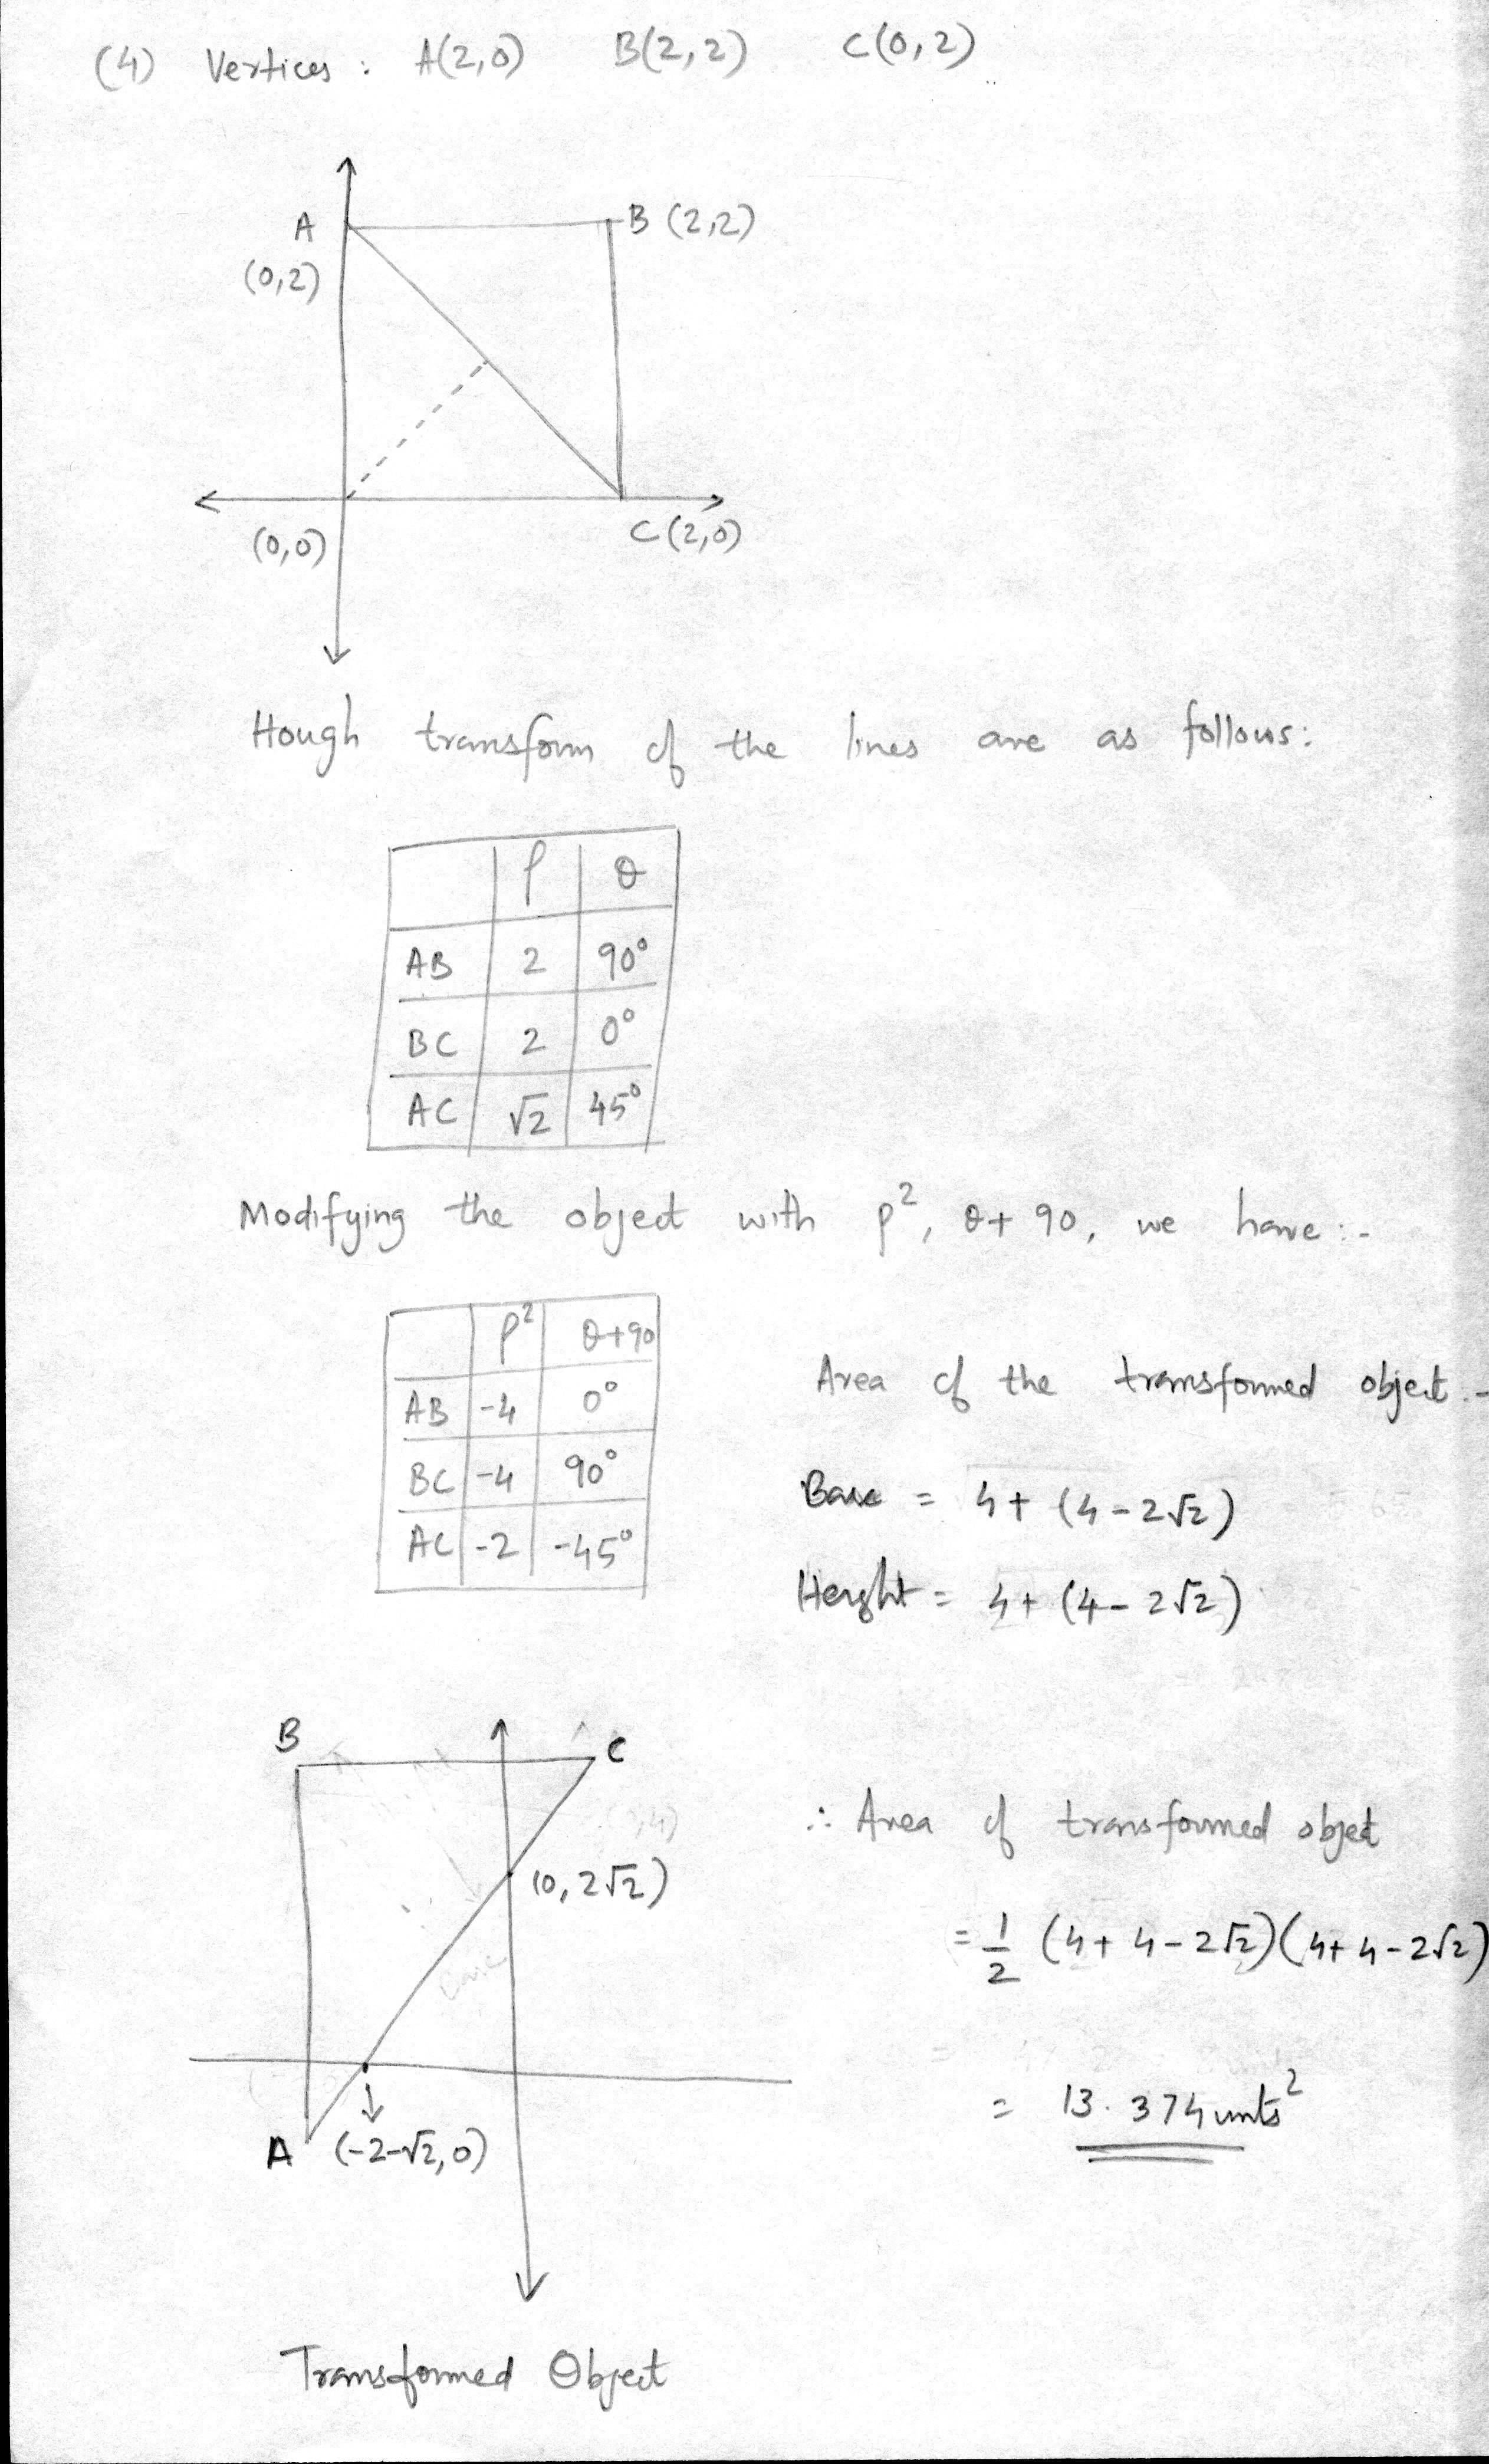
\includegraphics[width=17cm]{qn4.jpg}
\end{figure}

\begin{figure}
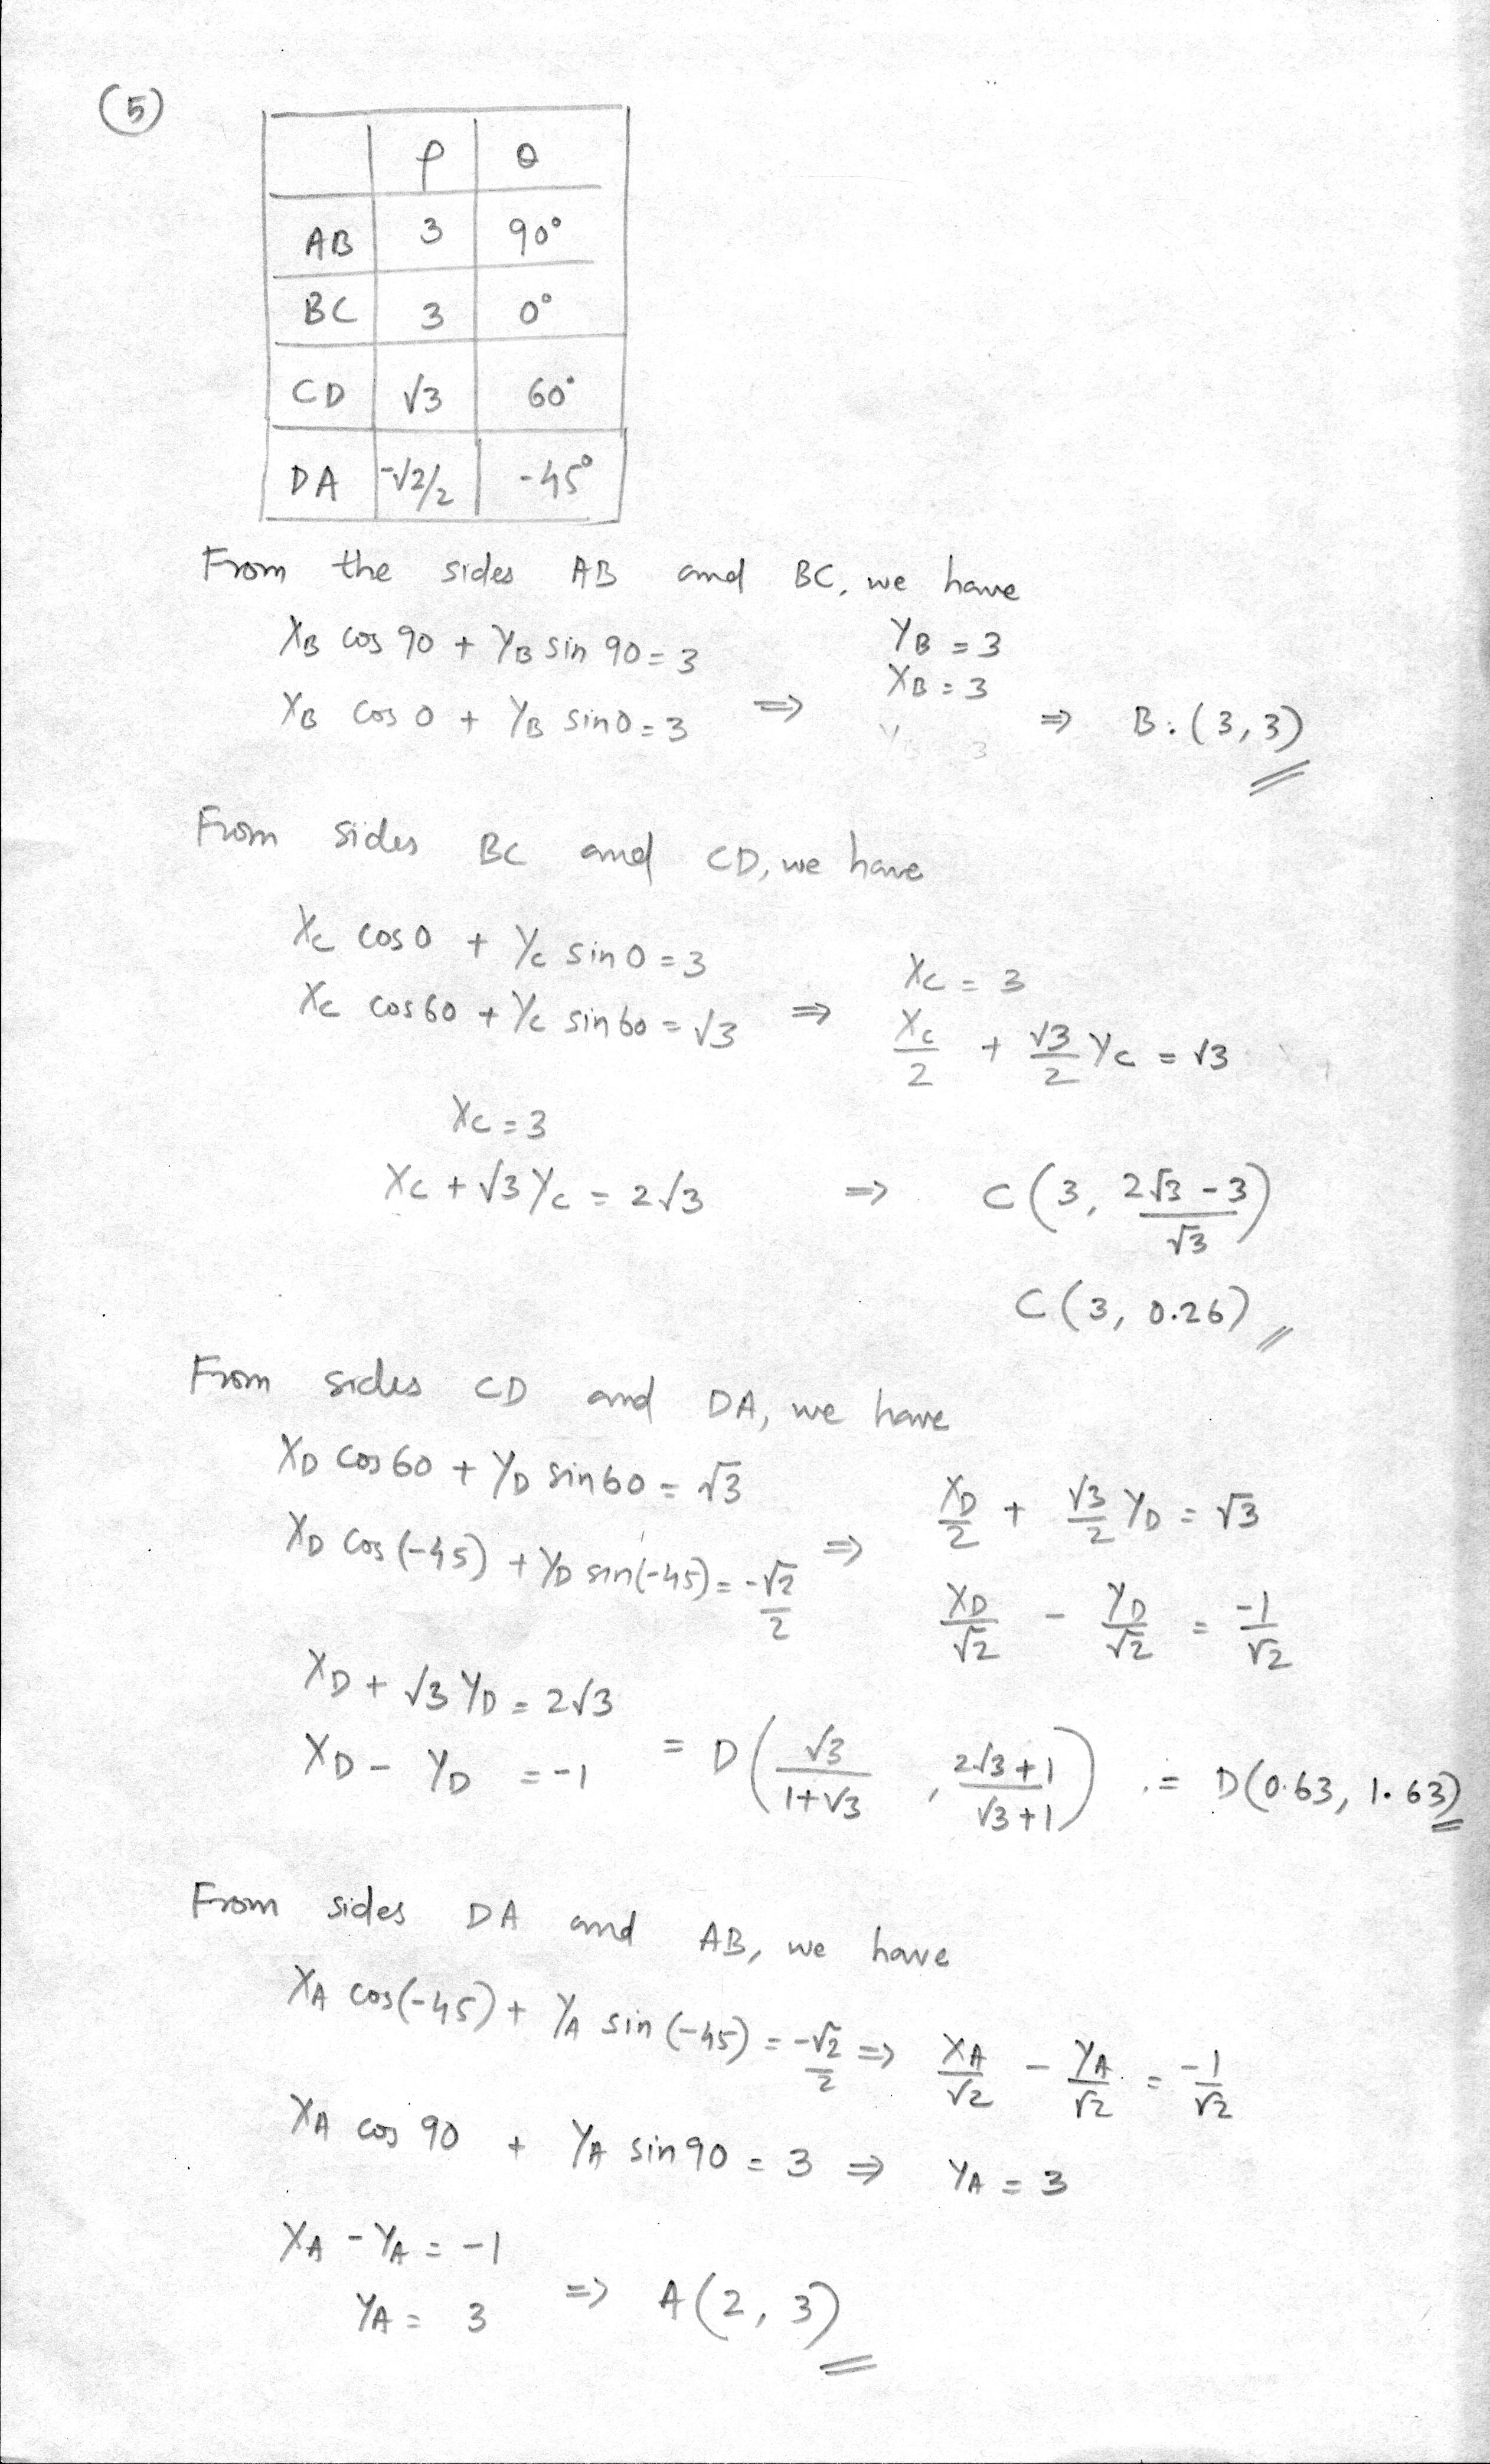
\includegraphics[width=15cm]{qn5_1.jpg}
\end{figure}

\begin{figure}
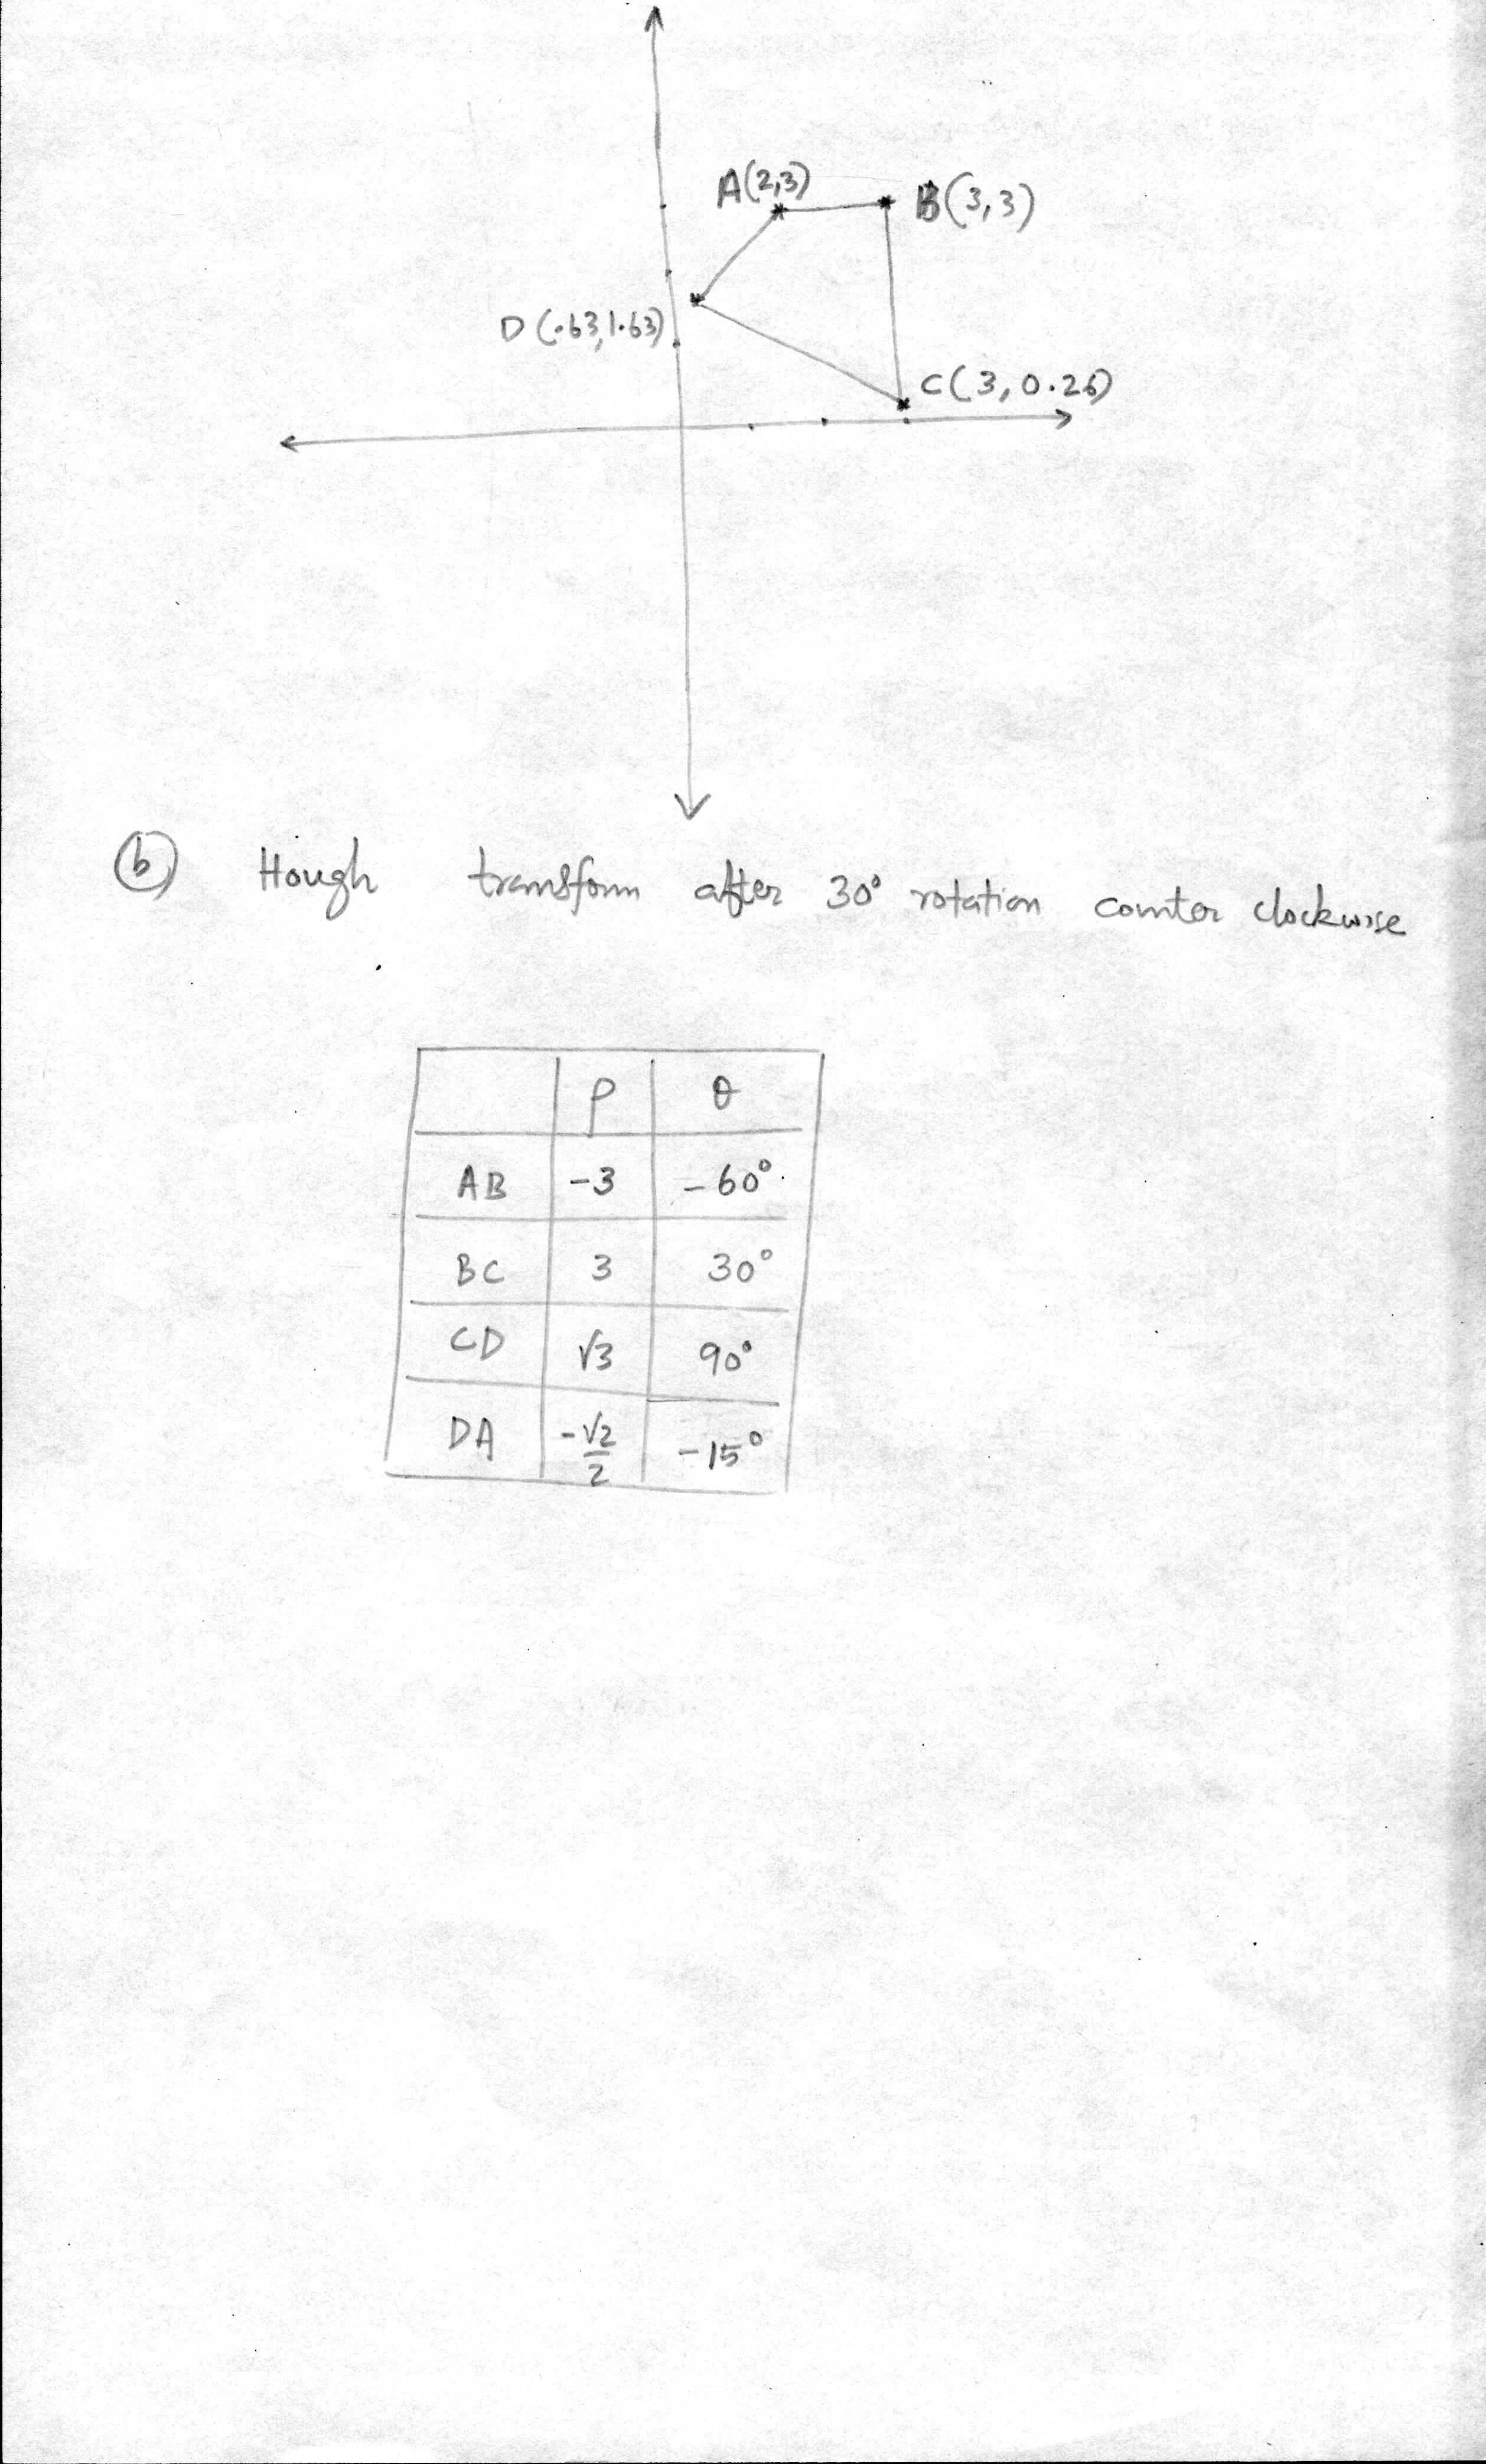
\includegraphics[width=15cm]{qn5_2.jpg}
\end{figure}

\begin{figure}
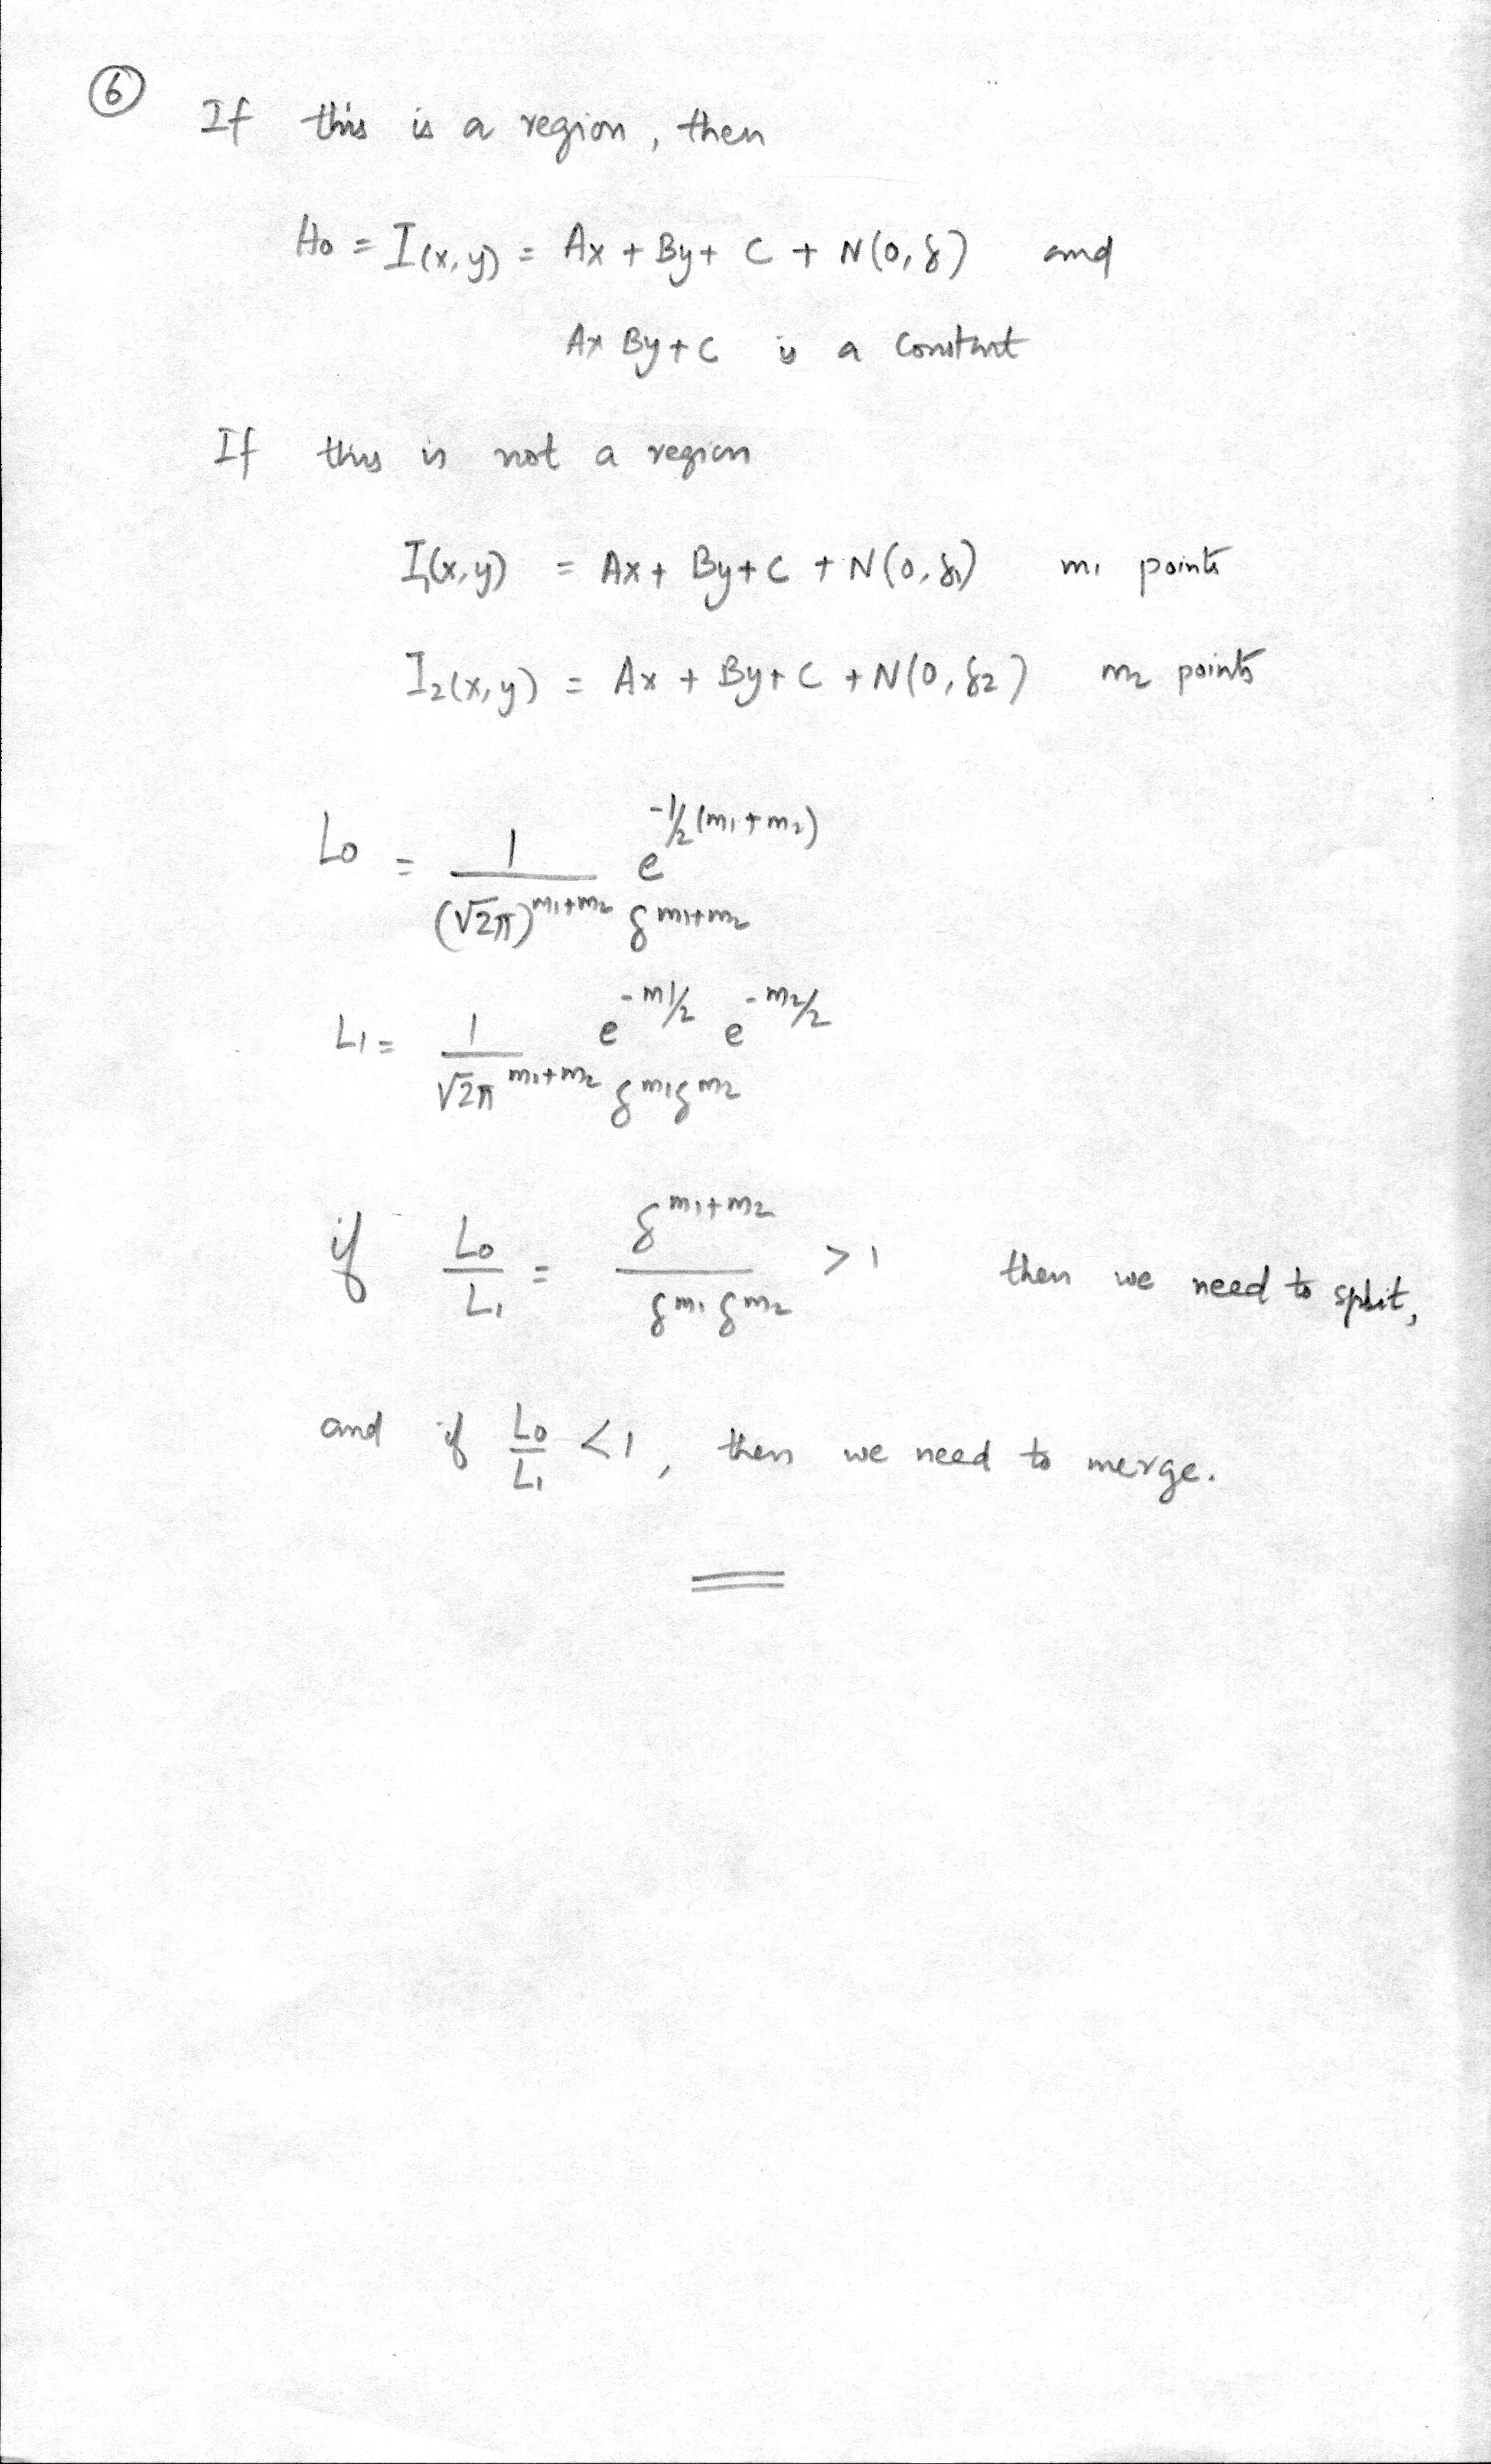
\includegraphics[width=15cm]{qn6.jpg}
\end{figure}

\begin{figure}
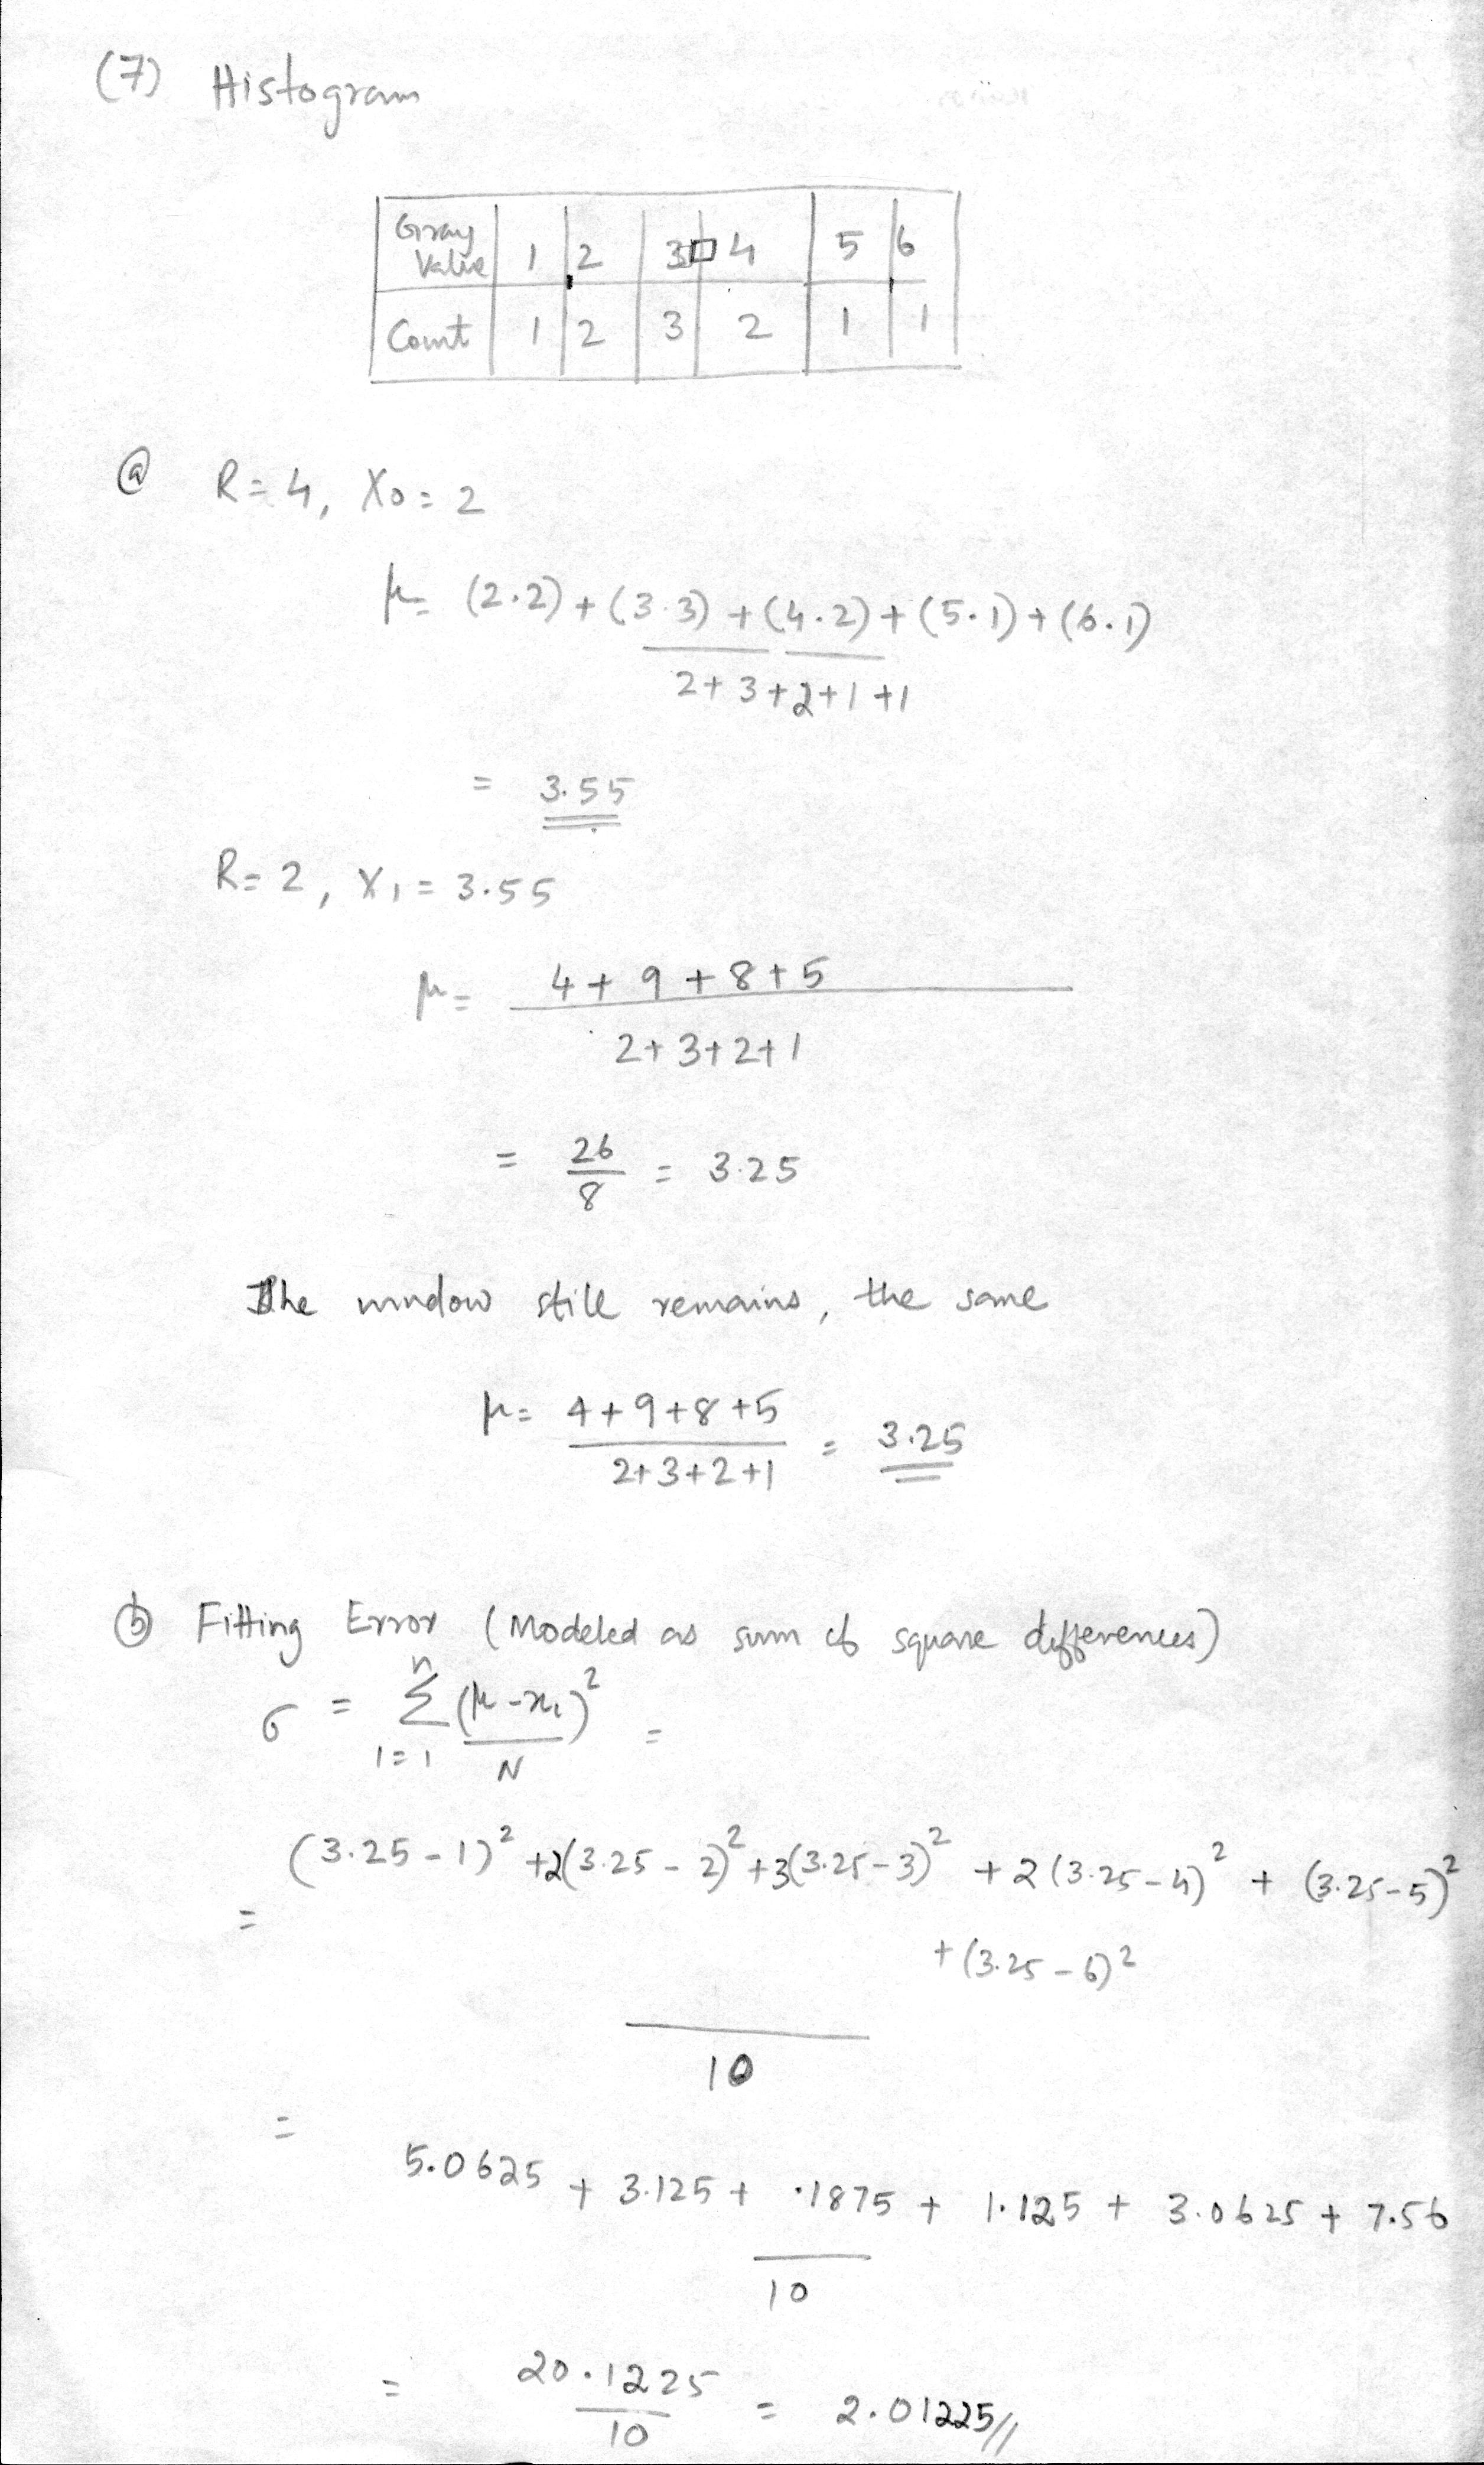
\includegraphics[width=15cm]{qn7_1.jpg}
\end{figure}

\begin{figure}
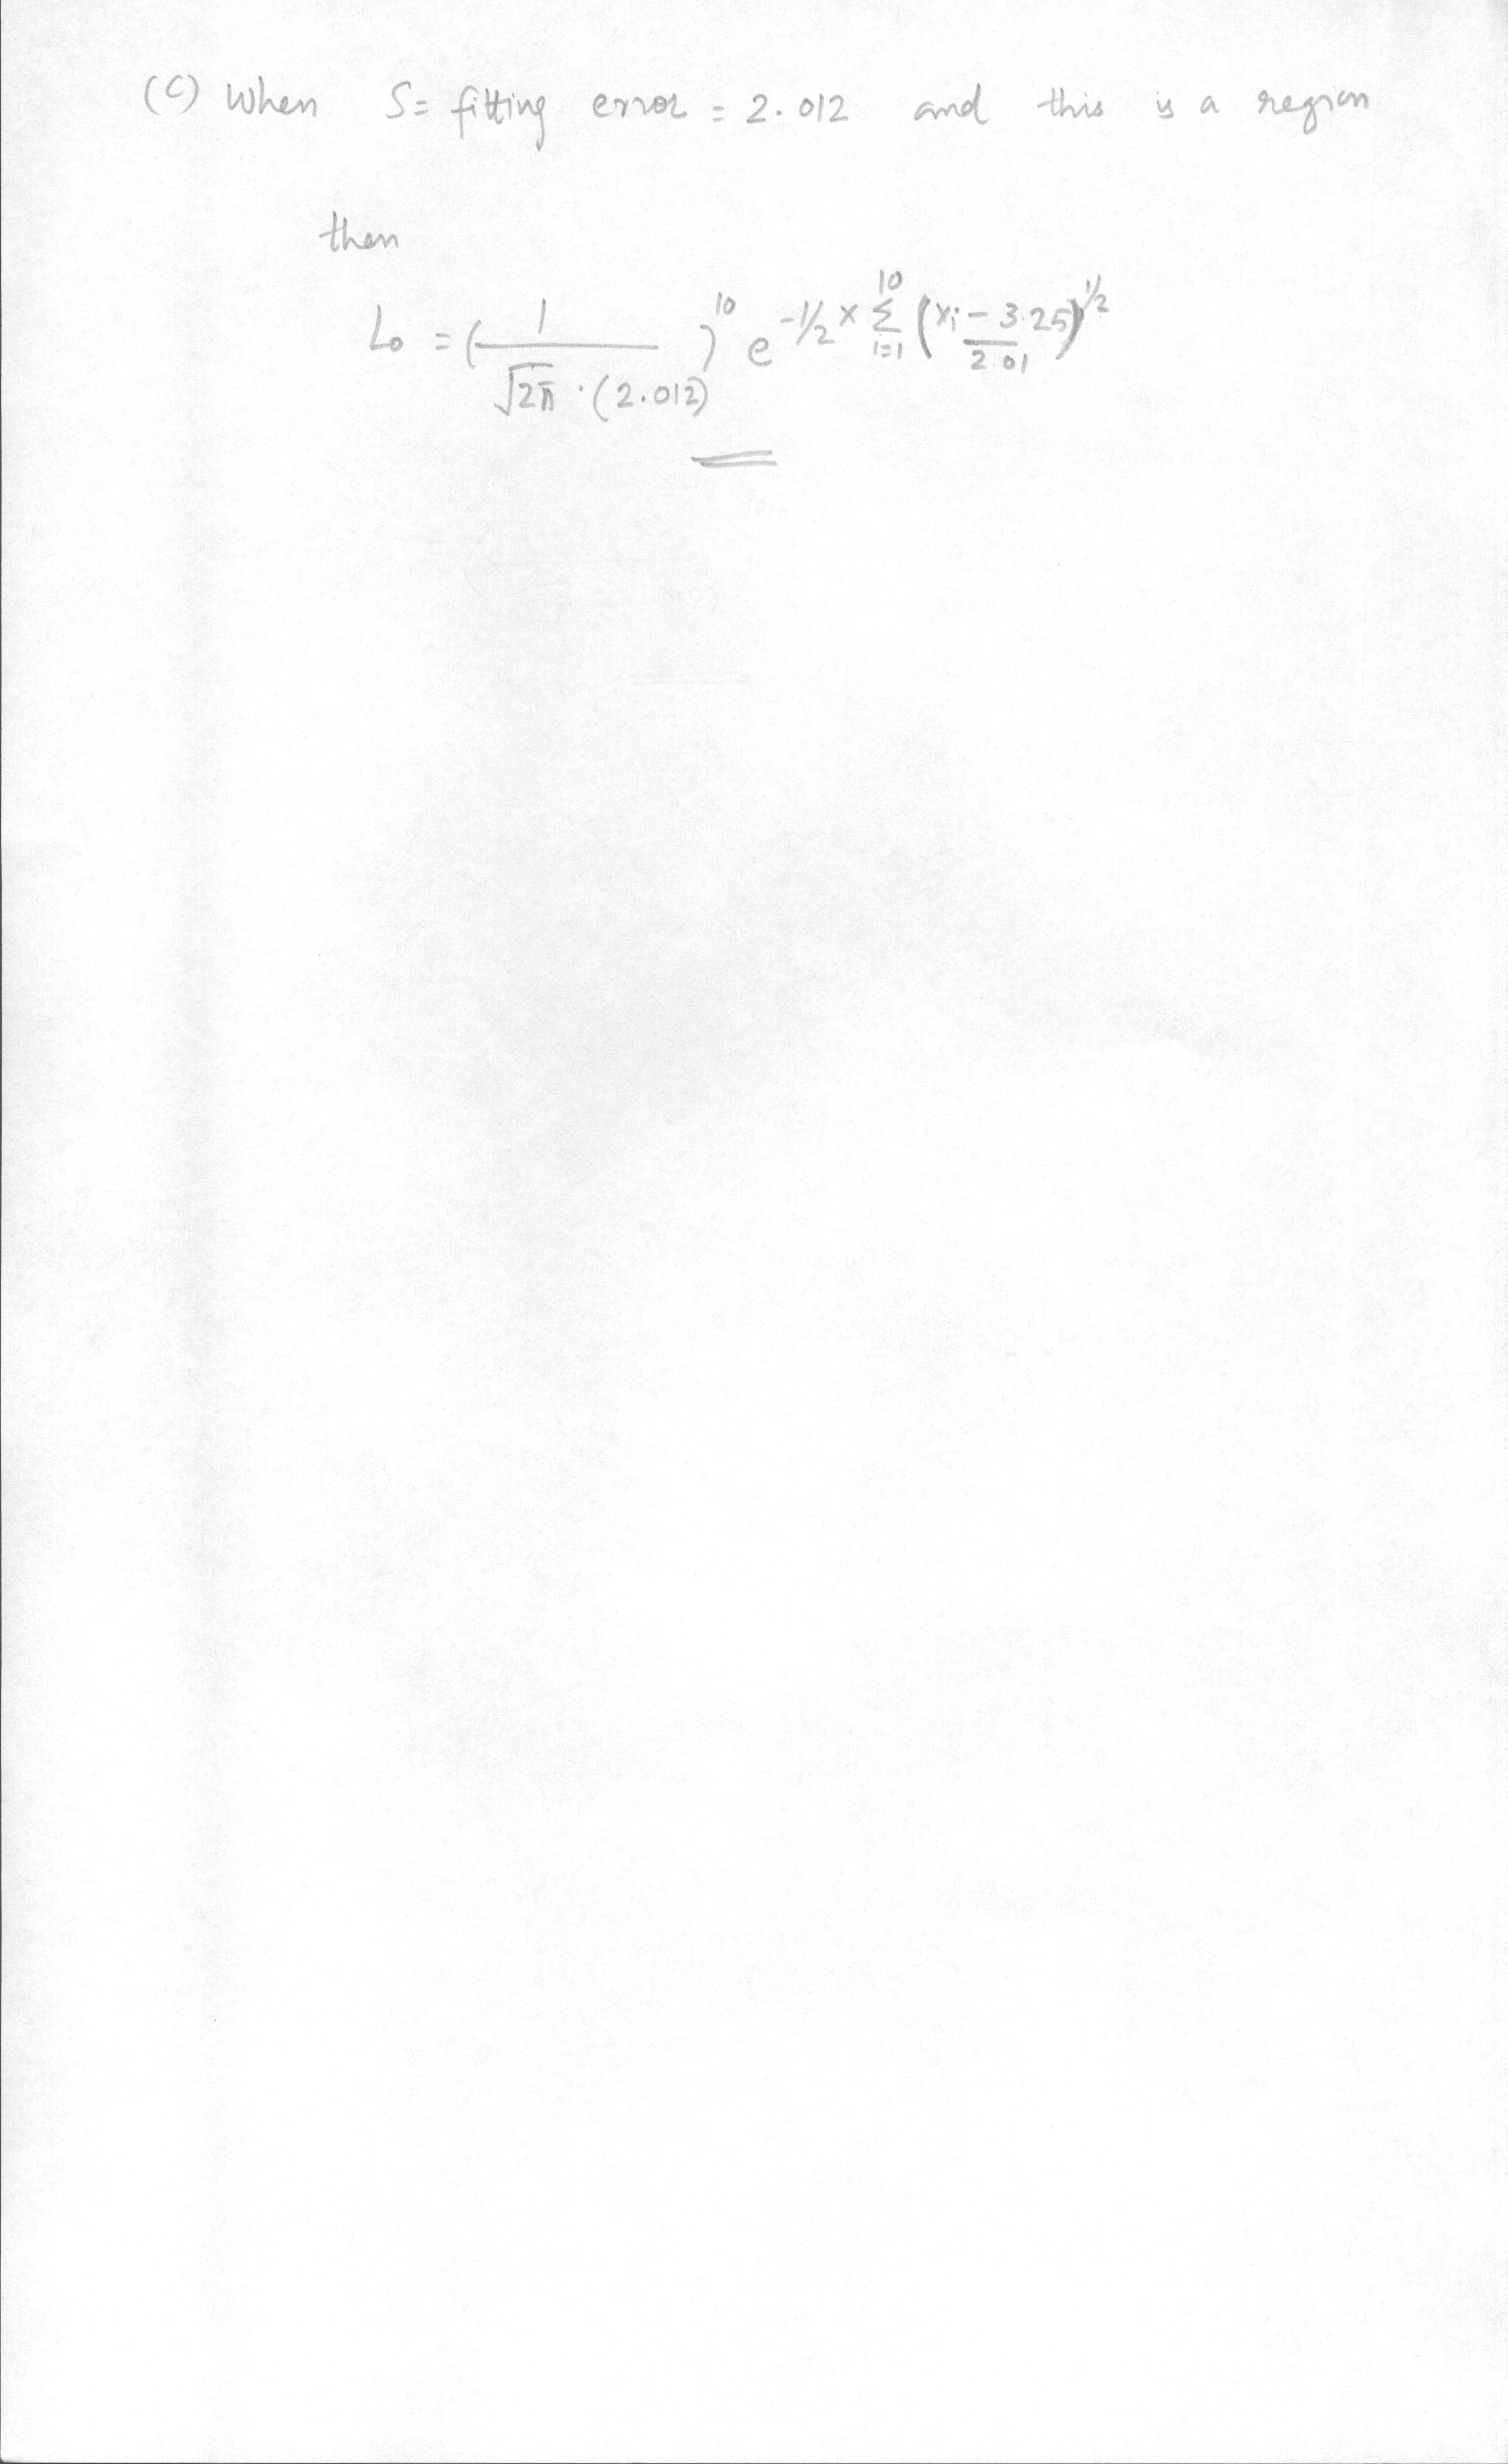
\includegraphics[width=15cm]{qn7_2.jpg}
\end{figure}



\end{document}

